% !TEX program = xelatex
\documentclass[11pt,a4paper]{article}

\usepackage[UTF8]{ctex}
\usepackage[margin=2.2cm]{geometry}
\usepackage{amsmath, amssymb, amsthm}
\usepackage{listings}
\usepackage{xcolor}
\usepackage{tikz}
\usepackage{booktabs}
\usepackage{multirow}
\usepackage{hyperref}
\usetikzlibrary{positioning, arrows.meta, shapes.geometric, fit, calc, decorations.pathreplacing}

\hypersetup{
  colorlinks=true,
  linkcolor=blue!60!black,
  urlcolor=teal!70!black,
}

\lstdefinelanguage{Rust}{
  morekeywords={fn,let,mut,pub,struct,impl,use,mod,self,Self,Option,Some,None,return,if,else,for,while,loop,match,break,continue,as,where,trait,type,enum,move,ref,const,static,unsafe,extern,crate,super,dyn,async,await,box,in},
  sensitive=true,
  morecomment=[l]{//},
  morecomment=[s]{/*}{*/},
  morestring=[b]",
}

\lstset{
  language=Rust,
  basicstyle=\ttfamily\footnotesize,
  keywordstyle=\color{blue!60!black}\bfseries,
  commentstyle=\color{green!40!black}\itshape,
  stringstyle=\color{red!60!black},
  numbers=left,
  numberstyle=\tiny\color{gray},
  numbersep=8pt,
  frame=single,
  framerule=0.4pt,
  rulecolor=\color{gray!40},
  breaklines=true,
  breakatwhitespace=true,
  showstringspaces=false,
  tabsize=4,
  columns=fullflexible,
  keepspaces=true,
}

\title{\textbf{halfedge\,: 链式查询 DSL 设计文档} \\ \large \texttt{src/query.rs}}
\author{halfedge 库}
\date{2026-07-04}

\begin{document}
\maketitle
\tableofcontents

\section{模块定位}

\texttt{query.rs} 在 \texttt{storage.rs} 之上叠加\textbf{链式查询}能力，
灵感来自 SMesh 和 OpenMesh 的 Builder 模式查询接口。

核心思路：为 \texttt{VertexId} 和 \texttt{HalfEdgeId} 提供一组返回
\texttt{MeshQuery<T>} 的方法，每个方法返回一个新的 \texttt{MeshQuery}，
捕获前序查询的闭包，在 \texttt{.run(\&mesh)} 时一次性求值整条链。

\begin{center}
\begin{tikzpicture}[
  node distance=0.35cm,
  box/.style={draw, rounded corners=3pt, minimum width=2.7cm, minimum height=0.9cm, align=center, font=\footnotesize},
  arrow/.style={-Stealth, thick, draw=blue!60!black}
]
  \node[box, fill=blue!10] (v) {\texttt{v0.halfedge\_to(v1)}};
  \node[box, fill=blue!10, right=of v] (cw) {\texttt{.cw\_rotated()}};
  \node[box, fill=blue!10, right=of cw] (dst) {\texttt{.dst\_vert()}};
  \node[box, fill=green!15, right=of dst] (run) {\texttt{.run(\&mesh)}};
  \node[box, fill=yellow!20, right=of run] (res) {\texttt{Option<VertexId>}};

  \draw[arrow] (v) -- (cw);
  \draw[arrow] (cw) -- (dst);
  \draw[arrow] (dst) -- (run);
  \draw[arrow] (run) -- (res);

  \node[below=0.25cm of v, font=\scriptsize, gray] {构造闭包 1};
  \node[below=0.25cm of cw, font=\scriptsize, gray] {包装闭包 2};
  \node[below=0.25cm of dst, font=\scriptsize, gray] {包装闭包 3};
  \node[below=0.25cm of run, font=\scriptsize, gray] {执行};
\end{tikzpicture}
\end{center}

\section{MeshQuery<T> 核心结构}

\subsection{数据结构}

\begin{lstlisting}
#[must_use]
pub struct MeshQuery<T> {
    f: Box<dyn FnOnce(&MeshStorage) -> Option<T>>,
}
\end{lstlisting}

\texttt{MeshQuery<T>} 内部存储一个 \texttt{FnOnce} 闭包，接收 \texttt{\&MeshStorage}
并返回 \texttt{Option<T>}。闭包在构造时不执行，只在 \texttt{.run()} 时求值。

\paragraph{\texttt{\#[must\_use]} 属性}
结构体标注 \texttt{\#[must\_use]} 后，任何返回 \texttt{MeshQuery<T>} 却未被消费
（未调用 \texttt{.run()} 或链式方法）的值都会触发编译器警告。这可防止用户
\textbf{忘记 \texttt{.run()}} 导致静默丢弃查询：
\begin{lstlisting}
// 警告：unused MeshQuery that must be used
v0.halfedge_to(v1).cw_rotated();          // 忘记 .run(&mesh)

// 正确：查询链以 .run() 终止
let nb = v0.halfedge_to(v1).cw_rotated().dst_vert().run(&mesh);
\end{lstlisting}
所有 \texttt{HalfEdgeId} / \texttt{VertexId} 直接方法与 \texttt{MeshQuery<T>}
链式方法均返回 \texttt{MeshQuery<T>}，因此均受此属性覆盖。

\subsection{三个核心方法}

\begin{center}
\renewcommand{\arraystretch}{1.20}
\begin{tabular}{@{}lll@{}}
  \toprule
  \textbf{方法} & \textbf{签名} & \textbf{语义} \\
  \midrule
  \texttt{new(f)} & \texttt{F: FnOnce(\&MeshStorage) -> Option<T>} & 从闭包构造查询 \\
  \texttt{run(mesh)} & \texttt{self -> Option<T>} & 执行查询链，消费 \texttt{self} \\
  \texttt{then(f)} & \texttt{(self, F) -> MeshQuery<U>} & 内部组合子：链接下一步 \\
  \bottomrule
\end{tabular}
\end{center}

\texttt{then} 是内部组合子，实现链式调用的核心：
\begin{lstlisting}
fn then<F, U>(self, f: F) -> MeshQuery<U>
where
    F: FnOnce(&MeshStorage, T) -> Option<U> + 'static,
    U: 'static,
{
    let prev = self.f;
    MeshQuery::new(move |mesh| {
        let val = prev(mesh)?;   // 前序查询
        f(mesh, val)             // 当前步骤
    })
}
\end{lstlisting}

关键语义：前序闭包返回 \texttt{None} 时，\texttt{?} 运算符\textbf{短路}，
后续步骤不执行，最终返回 \texttt{None}。

\section{方法一览}

\subsection{HalfEdgeId 方法}

\begin{center}
\renewcommand{\arraystretch}{1.18}
\begin{tabular}{@{}lll@{}}
  \toprule
  \textbf{方法} & \textbf{返回类型} & \textbf{拓扑操作} \\
  \midrule
  \texttt{twin()}       & \texttt{MeshQuery<HalfEdgeId>} & $h \mapsto h.\mathrm{twin}$ \\
  \texttt{next()}       & \texttt{MeshQuery<HalfEdgeId>} & $h \mapsto h.\mathrm{next}$ \\
  \texttt{prev()}       & \texttt{MeshQuery<HalfEdgeId>} & $h \mapsto h.\mathrm{prev}$ \\
  \texttt{face()}       & \texttt{MeshQuery<FaceId>}     & $h \mapsto h.\mathrm{face}$ \\
  \texttt{src\_vert()}  & \texttt{MeshQuery<VertexId>}   & $h \mapsto h.\mathrm{twin}.\mathrm{vertex}$（origin） \\
  \texttt{dst\_vert()}  & \texttt{MeshQuery<VertexId>}   & $h \mapsto h.\mathrm{vertex}$（tip） \\
  \texttt{cw\_rotated()}  & \texttt{MeshQuery<HalfEdgeId>} & $h \mapsto h.\mathrm{twin}.\mathrm{next}$ \\
  \texttt{ccw\_rotated()} & \texttt{MeshQuery<HalfEdgeId>} & $h \mapsto h.\mathrm{prev}.\mathrm{twin}$ \\
  \bottomrule
\end{tabular}
\end{center}

\subsection{VertexId 方法}

\begin{center}
\renewcommand{\arraystretch}{1.18}
\begin{tabular}{@{}lll@{}}
  \toprule
  \textbf{方法} & \textbf{返回类型} & \textbf{语义} \\
  \midrule
  \texttt{halfedge()}       & \texttt{MeshQuery<HalfEdgeId>} & 取 $v$ 的 outgoing 入口 \\
  \texttt{halfedge\_to(w)}  & \texttt{MeshQuery<HalfEdgeId>} & 遍历 outgoing 环找 $\mathrm{tip}=w$ 的半边 \\
  \bottomrule
\end{tabular}
\end{center}

\subsection{MeshQuery<T> 链式方法}

\texttt{MeshQuery<HalfEdgeId>}、\texttt{MeshQuery<VertexId>} 与
\texttt{MeshQuery<FaceId>} 各自实现与对应 ID 类型相同的方法集，通过
\texttt{then} 组合子链接前序查询与当前步骤。

\begin{center}
\renewcommand{\arraystretch}{1.20}
\scriptsize
\begin{tabular}{@{}ll@{}}
  \toprule
  \textbf{MeshQuery<T>} & \textbf{可用方法} \\
  \midrule
  \texttt{MeshQuery<HalfEdgeId>} & \texttt{twin / next / prev / face} \\
                                 & \texttt{src\_vert / dst\_vert} \\
                                 & \texttt{cw\_rotated / ccw\_rotated} \\
  \texttt{MeshQuery<VertexId>}   & \texttt{halfedge / halfedge\_to} \\
  \texttt{MeshQuery<FaceId>}     & \texttt{halfedge}（取面入口半边，转入 HalfEdgeId 链） \\
  \bottomrule
\end{tabular}
\end{center}

\section{CW / CCW 旋转规则}

\subsection{几何图示}

\begin{center}
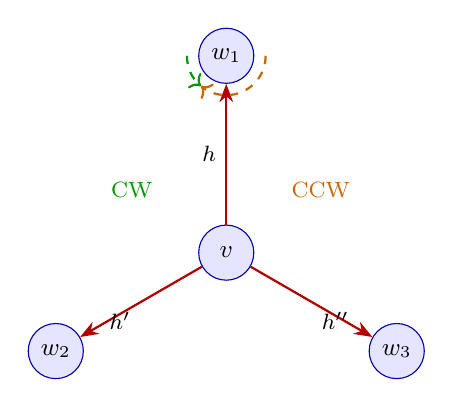
\begin{tikzpicture}[
  vert/.style={circle, draw=blue!70!black, fill=blue!10, minimum size=7mm, inner sep=0pt, font=\small},
  he/.style={-Stealth, thick, draw=red!70!black},
  rot/.style={->, thick, dashed, draw=orange!80!black}
]
  % 中心顶点 v
  \node[vert] (v) at (0,0) {$v$};
  % 周围三个邻居
  \node[vert] (w1) at (90:2.5)  {$w_1$};
  \node[vert] (w2) at (210:2.5) {$w_2$};
  \node[vert] (w3) at (330:2.5) {$w_3$};

  % 三条 outgoing 半边
  \draw[he] (v) -- node[left, font=\footnotesize] {$h$} (w1);
  \draw[he] (v) -- node[below left, font=\footnotesize] {$h'$} (w2);
  \draw[he] (v) -- node[below right, font=\footnotesize] {$h''$} (w3);

  % CCW 旋转箭头（h → h'）
  \draw[rot] ($(w1)+(0.5,0.0)$) arc[start angle=0, end angle=-130, radius=0.5];
  \node[font=\footnotesize, orange!80!black] at (1.2, 0.8) {CCW};

  % CW 旋转箭头（h → h''）
  \draw[rot, draw=green!60!black] ($(w1)+(-0.5,0.0)$) arc[start angle=180, end angle=230, radius=0.5];
  \node[font=\footnotesize, green!60!black] at (-1.2, 0.8) {CW};
\end{tikzpicture}
\end{center}

\subsection{公式推导}

设 $h$ 是顶点 $v$ 的 outgoing 半边（$h.\mathrm{twin}.\mathrm{vertex} = v$）：

\textbf{CW 旋转}（顺时针绕 $v$ 到相邻面）：
\[
\mathrm{cw\_rotated}(h) = h.\mathrm{twin}.\mathrm{next}
\]
推导：$h.\mathrm{twin}$ 结尾落在 $v$；其 $\mathrm{next}$ 起始于 $v$，
属于 $h$ 顺时针方向的相邻面。

\textbf{CCW 旋转}（逆时针绕 $v$ 到相邻面）：
\[
\mathrm{ccw\_rotated}(h) = h.\mathrm{prev}.\mathrm{twin}
\]
推导：$h.\mathrm{prev}$ 与 $h$ 同面，结尾落在 $v$；其 $\mathrm{twin}$
起始于 $v$，属于 $h$ 逆时针方向的相邻面。

\section{链式求值流程}

\begin{center}
\resizebox{\textwidth}{!}{%
\begin{tikzpicture}[
  node distance=0.55cm,
  proc/.style={draw, rounded corners=2pt, minimum width=10cm, minimum height=0.7cm, align=center, font=\small},
  dec/.style={diamond, draw, aspect=2.4, fill=orange!12, inner sep=1pt, font=\small, align=center, minimum width=4cm},
  op/.style={-Stealth, thick},
  startend/.style={draw, rounded corners=10pt, minimum width=2.6cm, minimum height=0.7cm, font=\small, fill=gray!12}
]
  \node[startend] (s) {调用 \texttt{.run(\&mesh)}};
  \node[proc, below=of s, fill=blue!8] (p1) {执行闭包 1：$r_1 \gets f_1(\mathrm{mesh})$};
  \node[dec, below=of p1] (d1) {$r_1$ 是否为 \texttt{Some}？};
  \node[proc, below=of d1, fill=blue!8] (p2) {执行闭包 2：$r_2 \gets f_2(\mathrm{mesh}, r_1)$};
  \node[dec, below=of p2] (d2) {$r_2$ 是否为 \texttt{Some}？};
  \node[proc, below=of d2, fill=blue!8] (p3) {执行闭包 3：$r_3 \gets f_3(\mathrm{mesh}, r_2)$};
  \node[proc, below=of p3, fill=green!12] (p4) {$\cdots$ 继续直到链末};
  \node[startend, below=of p4, fill=green!12] (ok) {返回 \texttt{Some(最终结果)}};
  \node[startend, right=2.5cm of d1, fill=red!10] (none1) {返回 \texttt{None}（短路）};
  \node[startend, right=2.5cm of d2, fill=red!10] (none2) {返回 \texttt{None}（短路）};

  \draw[op] (s) -- (p1);
  \draw[op] (p1) -- (d1);
  \draw[op] (d1) -- node[right, font=\footnotesize] {是} (p2);
  \draw[op] (d1) -- node[above, near start, font=\footnotesize] {否} (none1);
  \draw[op] (p2) -- (d2);
  \draw[op] (d2) -- node[right, font=\footnotesize] {是} (p3);
  \draw[op] (d2) -- node[above, near start, font=\footnotesize] {否} (none2);
  \draw[op] (p3) -- (p4);
  \draw[op] (p4) -- (ok);
\end{tikzpicture}%
}
\end{center}

\textbf{短路语义}：链中任一环节返回 \texttt{None}，后续闭包不执行，
最终返回 \texttt{None}。这保证了无效 ID、边界半边等场景下的安全行为。

\section{示例查询}

\subsection{用户示例：两三角形共享边上的 CW 旋转}

\begin{lstlisting}
// 两三角形拼成四边形，共享边 v0-v1
// v0.halfedge_to(v1) = h0 (v0→v1, 共享边)
// h0.cw_rotated() = twin(h0).next = g0.next = g1 (v0→v3)
// g1.dst_vert() = v3
let neighbor = v0.halfedge_to(v1)
    .cw_rotated()
    .dst_vert()
    .run(&mesh);
assert_eq!(neighbor, Some(v3));
\end{lstlisting}

\begin{center}
\begin{tikzpicture}[
  vert/.style={circle, draw=blue!70!black, fill=blue!10, minimum size=7mm, inner sep=0pt, font=\small},
  he/.style={-Stealth, thick, draw=red!70!black},
  he2/.style={-Stealth, thick, draw=green!60!black},
  lab/.style={font=\footnotesize, sloped, above}
]
  \node[vert] (v0) at (0,0)    {$v_0$};
  \node[vert] (v1) at (3,0)    {$v_1$};
  \node[vert] (v2) at (0,2.5)  {$v_2$};
  \node[vert] (v3) at (3,-2.5) {$v_3$};

  % F1: v0→v1→v2→v0 (CCW，位于共享边上方)
  \draw[he] (v0) -- node[lab] {$h_0$} (v1);
  \draw[he] (v1) -- node[lab] {$h_1$} (v2);
  \draw[he] (v2) -- (v0);
  % F2: v1→v0→v3→v1 (CCW，位于共享边下方)
  \draw[he2] (v0) -- node[lab] {$g_1$} (v3);
  \draw[he2] (v3) -- (v1);
  % g0 是 h0 的 twin（v1→v0），省略

  % CW 旋转弧线：h0 → g1（绕 v0 顺时针，从 +x 方向到 -y 方向）
  \draw[->, thick, dashed, draw=orange!80!black]
    ($(v0)+(0.7,0)$) arc[start angle=0, end angle=-50, radius=0.7];
  \node[font=\footnotesize, orange!80!black] at (0.9, -0.6) {CW};

  \node[font=\footnotesize, align=center] at (1.5, -3.4)
    {链：$h_0 \xrightarrow{\text{cw}} g_1 \xrightarrow{\text{dst}} v_3$};
\end{tikzpicture}
\end{center}

\subsection{闭合扇形上的连续旋转}

\begin{lstlisting}
// 中心 c 被 3 个面环绕（闭合环）
// a1: c→v0, cw_rotated(a1) = a3 (c→v2)
// 连续 CW 旋转 3 次回到 a1
let result = a1.cw_rotated()
    .cw_rotated()
    .cw_rotated()
    .run(&mesh);
assert_eq!(result, Some(a1));

// CCW 旋转同样闭合
let result = a1.ccw_rotated()
    .ccw_rotated()
    .ccw_rotated()
    .run(&mesh);
assert_eq!(result, Some(a1));
\end{lstlisting}

\subsection{面边界环遍历}

\begin{lstlisting}
// h0.next().next().next() 应回到 h0（闭合面环）
assert_eq!(h0.next().next().next().run(&mesh), Some(h0));

// h0.next().dst_vert() = h1.vertex = v2
assert_eq!(h0.next().dst_vert().run(&mesh), Some(v2));
\end{lstlisting}

\subsection{src/dst 往返查询}

\begin{lstlisting}
// h0.src_vert() = v0, v0.halfedge_to(v1) = h0
// 应找回原始半边
assert_eq!(
    h0.src_vert().halfedge_to(v1).run(&mesh),
    Some(h0)
);
\end{lstlisting}

\section{健壮性}

\begin{itemize}
  \item \textbf{无效 / 已删除 ID}：所有方法依赖 \texttt{mesh.get\_halfedge} /
        \texttt{mesh.get\_vertex}，返回 \texttt{None} 时链短路，不 panic。
  \item \textbf{边界半边}：\texttt{twin.next} 或 \texttt{prev.twin} 撞到
        \texttt{None} 时，\texttt{cw\_rotated} / \texttt{ccw\_rotated} 返回 \texttt{None}。
  \item \textbf{短路保护}：链中任一环节 \texttt{None}，后续闭包不执行，
        避免 \texttt{unwrap} / 空指针。
  \item \texttt{halfedge\_to} 复用 \texttt{traversal::VertexRingLazy}，
        正确处理闭合环与开链，以半边总数加一为上界防止死循环。
\end{itemize}

\section{内部辅助函数}

每个半边操作都抽取为独立的辅助函数，被 \texttt{HalfEdgeId} 直接方法和
\texttt{MeshQuery<HalfEdgeId>} 链式方法\textbf{共用}，消除代码重复：

\begin{center}
\renewcommand{\arraystretch}{1.18}
\begin{tabular}{@{}ll@{}}
  \toprule
  \textbf{辅助函数} & \textbf{实现} \\
  \midrule
  \texttt{he\_twin(mesh, he)}    & \texttt{mesh.get\_halfedge(he).and\_then(|h| h.twin)} \\
  \texttt{he\_next(mesh, he)}    & \texttt{mesh.get\_halfedge(he).and\_then(|h| h.next)} \\
  \texttt{he\_prev(mesh, he)}    & \texttt{mesh.get\_halfedge(he).and\_then(|h| h.prev)} \\
  \texttt{he\_face(mesh, he)}    & \texttt{mesh.get\_halfedge(he).and\_then(|h| h.face)} \\
  \texttt{he\_src\_vert(mesh, he)} & \texttt{get(he).twin → get → .vertex} \\
  \texttt{he\_dst\_vert(mesh, he)} & \texttt{get(he) → .vertex} \\
  \texttt{he\_cw\_rotated(mesh, he)} & \texttt{get(he).twin → get → .next} \\
  \texttt{he\_ccw\_rotated(mesh, he)} & \texttt{get(he).prev → get → .twin} \\
  \texttt{vertex\_halfedge(mesh, v)} & \texttt{get\_vertex(v).and\_then(|vt| vt.halfedge)} \\
  \texttt{vertex\_halfedge\_to(mesh, v, w)} & \texttt{VertexRingLazy::new(mesh, v).find(...)} \\
  \texttt{face\_halfedge(mesh, f)} & \texttt{get\_face(f).and\_then(|fc| fc.halfedge)} \\
  \bottomrule
\end{tabular}
\end{center}

\section{单元测试覆盖}

\texttt{src/query.rs} 末尾共 19 个测试，分五组：

\begin{center}
\scriptsize
\renewcommand{\arraystretch}{1.18}
\begin{tabular}{@{}ll@{}}
  \toprule
  \textbf{测试名} & \textbf{覆盖点} \\
  \midrule
  \multicolumn{2}{l}{\textit{基本查询：VertexId}} \\
  \texttt{vertex\_halfedge\_query}              & \texttt{v.halfedge().run()} 取 outgoing 入口 \\
  \texttt{vertex\_halfedge\_to\_finds\_correct\_edge} & \texttt{v.halfedge\_to(w)} 找正确半边 + 不存在邻居 \\
  \midrule
  \multicolumn{2}{l}{\textit{基本查询：HalfEdgeId}} \\
  \texttt{halfedge\_twin\_query}                & twin 互指 \\
  \texttt{halfedge\_next\_prev\_query}          & 面 CCW 环 next/prev \\
  \texttt{halfedge\_face\_query}                & 面内 → Some(f)，边界 twin → None \\
  \texttt{halfedge\_src\_dst\_vert\_query}      & origin / tip 取顶点 \\
  \texttt{halfedge\_rotation\_on\_closed\_fan}  & CW/CCW 旋转 + 连续 3 次闭合 \\
  \texttt{halfedge\_cw\_rotated\_boundary\_returns\_none} & 边界半边 CW 旋转 → None \\
  \midrule
  \multicolumn{2}{l}{\textit{基本查询：FaceId}} \\
  \texttt{face\_halfedge\_query}                & \texttt{f.halfedge().run()} 取面入口半边 \\
  \texttt{face\_query\_on\_invalid\_face\_returns\_none} & 无效 FaceId 返回 None \\
  \midrule
  \multicolumn{2}{l}{\textit{链式查询}} \\
  \texttt{chain\_user\_example\_on\_two\_triangles} & 用户示例：CW 旋转取邻居 \\
  \texttt{chain\_closed\_fan\_rotations}        & 闭合扇 CW/CCW 旋转取邻居 \\
  \texttt{chain\_traverses\_face\_boundary}     & next 链遍历面环 \\
  \texttt{chain\_src\_dst\_roundtrip}           & src\_vert → halfedge\_to 往返 \\
  \texttt{chain\_short\_circuits\_on\_none}     & 链中 None 短路 \\
  \texttt{meshquery\_face\_chain\_halfedge}     & \texttt{MeshQuery<FaceId>} 链式 \texttt{halfedge()} \\
  \texttt{face\_chained\_query}                 & FaceId 链式查询完整路径 \\
  \midrule
  \multicolumn{2}{l}{\textit{无效 / 已删除 ID}} \\
  \texttt{invalid\_ids\_return\_none}           & 孤立 / 已删除 / 默认 ID 全方法返回 None \\
  \texttt{chain\_on\_invalid\_ids\_short\_circuits} & 默认 ID 链式短路 \\
  \bottomrule
\end{tabular}
\end{center}

\texttt{cargo test} 全模块共 \textbf{371 个}用例，全部通过（0 失败 / 0 警告）。

\section{设计取舍}

\begin{itemize}
  \item \textbf{为何用 \texttt{Box<dyn FnOnce>} 而非泛型？} 泛型参数会在链中
        嵌套展开（每链一步增加一层 \texttt{Then<\ldots>} 包装），类型复杂度爆炸。
        \texttt{Box<dyn FnOnce>} 将类型擦除为单一 \texttt{MeshQuery<T>}，
        链长度不影响类型签名。
  \item \textbf{为何 \texttt{FnOnce} 而非 \texttt{FnMut}？} 每个方法消费 \texttt{self}，
        将前序闭包 \texttt{move} 进新闭包，是一次性操作。\texttt{FnOnce} 语义最精确。
  \item \textbf{为何用 \texttt{then} 组合子？} 半边操作的逻辑（如 \texttt{twin.next}
        用于 CW 旋转）在直接方法和链式方法中完全相同。\texttt{then} 将公共逻辑
        抽取为辅助函数，两处共用，消除重复。
  \item \textbf{为何 \texttt{MeshQuery<FaceId>} 仅提供 \texttt{halfedge}？}
        \texttt{FaceId} 在半边结构中只有「取面入口半边」一种 O(1) 操作。
        \texttt{f.halfedge().run(\&mesh)} 返回 \texttt{Option<HalfEdgeId>}，
        自然转入 \texttt{MeshQuery<HalfEdgeId>} 链继续查询。
\end{itemize}

\end{document}
